% Chapter Template

\chapter{Literature Review} % Main chapter title

\label{Chapter2} % Change X to a consecutive number; for referencing this chapter elsewhere, use \ref{ChapterX}

\lhead{Chapter 2. \emph{State of the Art}} % Change X to a consecutive number; this is for the header on each page - perhaps a shortened title

%----------------------------------------------------------------------------------------
%	SECTION 1
%----------------------------------------------------------------------------------------

\section{Introduction}

This section introduces fields of study under investigation in this project, Machine Learning and Argumentation Theory. The existing literature on both areas is reviewed in order to provide the reader with an understanding of the context in which the research occurs. As the project is fundamentally a comparison between the two fields this literature review also gathers results and conclusions from other work that will help to inform this comparison. This material will be used to support the arguments made for both approaches and will also inform the design of an experiment evaluating the approaches.
%-----------------------------------
%	MACHINE LEARNING
%-----------------------------------
\section{Machine Learning}

\cite{mitchell2006discipline} defines machine learning as a field of computer science that attempts to solve the question:

``How can we build computer systems that automatically improve with experience, and what are the fundamental laws that govern all learning processes?''

On a practical level it is an area of study that concerns itself with the design of techniques and algorithms that run uniquely on different data to achieve some aim without being explicitly programmed. A machine learning program initial takes a data as input which it learns from; this learning is then used on future inputs to make a prediction or to provide some understanding. Mitchell outlines that while there had been no successful commercial applications of machine learning as late as 1985, it has since been successfully applied in diverse fields such as speech recognition, computer vision, bio-surveillance, robot control and accelerating empirical sciences. Indeed in the last several years some of the biggest names in technology such as IBM, Google, Microsoft and Baidu have been making great strides in the development of advanced machine learning techniques and reaping the rewards.

The literature makes the distinction between different learning scenarios. \cite{alpaydinintroduction} explains that `supervised learning' happens in a scenario in which the task of the algorithm is to learn the mapping from some input X to an output Y. Examples \footnote{Taken from Kaggle.com; a website for data science competitions} of questions supervised learning attempts to answer include:

\begin{itemize}
  \item What is the probabilistic distribution of hourly rain given polarimetric radar measurements?
  \item What category does a particular product belong to given it's features?
  \item Given a number of objective measurements, what will be a restaurant's annual sales? 
\end{itemize}

In a review of supervised learning classification techniques, \cite{kotsiantis2007supervised} explains that if ``known labels (the corresponding correct outputs)" are used ``then the learning is called supervised". 

Supervised learning problems can be further divided into two categories; regression problems and classification problems. 
\cite{ng2000cs229} explains that regression problems are problems where the output to be predicted is continuous. In a regression problem as specific numeric value is predicted, for example, a restaurant's annual sales in the example above. Problems in which the output to be predicted is discrete are considered classification problems. Classification problems tend to be concerned with the sorting of data into correct categories, as in the second example above. Another such problem might be determining whether or not a particular email should be categorised as spam or not.  

Supervised learning can be contrasted with unsupervised learning; described by \cite{mohri2012foundations} as problems in which ``the learner receives unlabelled training data and makes predictions for all unseen points.'' The learning is called unsupervised because the techniques don't attempt to make predictions based on a specific labeled output. Instead unsupervised learning techniques are used to perform tasks such as identifying clusters in data, anomaly detection and dimensionality reduction. Examples of practical applications of unsupervised learning (taken from \cite{ng2000cs229}) are:

\begin{itemize}
  \item Organizing computer clusters.
  \item Social network analysis.
  \item Identification of market segments.
\end{itemize}

The following sections introduce the reader to machine learning techniques from each of the different categories at a high level. Many of the techniques outlined require a strong understanding of mathematics in order to fully understand and engage with them. This outline will avoid these details as explaining them sufficiently is beyond the scope of this project.

\section{Supervised Learning}


\section{Supervised Learning - Classification Techniques}

This section introduces common techniques used to solve classification problems.
% naivebayes
\subsection{Naive-Bayes}
\cite{kohavi1997improving} introduces Naive-Bayes or Simple-Bayesian Classifier and then outlines techniques for it's improvement. The learner is ``built based on a conditional independence model of each attribute given the class.'' Put simply the learner uses probability to classify the data. Bayes refers to Bayes rule, a mathematical rule for computing the probability that something happens given some other \textit{a priori} condition. The technique is called Naive as the probabilities of the features in the model are assumed to be independent. The probability of each class is computed for a row in the data set. The class with the highest probability for that row is the class that is chosen for that instance of the data.


\subsection{Bayesian Networks}

\cite{export:69588} explains that Bayesian Networks have been increasingly employed in expert systems as an encoding for an experts knowledge. One of the strengths of Bayesian Networks is that they can still produce an output with incomplete data. Bayesian Networks provide methods for dealing with uncertainty by graphically modelling dependent relationships. Each attribute is modelled as a vertex in the graph with the relationships modeled as edges. Internally the nodes have a table containing the probability outcomes given conditions have occurred in their parent nodes. In figure~\ref{fig:test}, an example taken from \cite{witten2005data} the probability of the temperature being hot, mild or cool depends on the values of play and outlook. The table appears as in table~\ref{fig:bayes_table}.

\begin{figure}[h]
\centering
\begin{tikzpicture}

\tikzset{vertex/.style = {shape=circle,draw,minimum size=1.5em}}
\tikzset{edge/.style = {->,> = latex'}}
% vertices

\node[vertex] (a) at  (3,0) {$play$};
\node[vertex] (b) at  (3,2) {$humidity$};
\node[vertex] (c) at  (2,4) {$temperature$};
\node[vertex] (d) at  (0,2) {$outlook$};
\node[vertex] (e) at  (0,0) {$windy$};

%edges

\draw[edge] (a) to (b);
\draw[edge] (a) to (c);
\draw[edge] (a) to (d);
\draw[edge] (a) to (e);
\draw[edge] (c) to (b);
\draw[edge] (d) to (c);
\draw[edge] (d) to (e);

\end{tikzpicture}
\caption{An example of a Bayesian Network from \cite{witten2005data}}
\label{fig:test}
\end{figure}

\begin{table}[h]
\centering
\begin{tabular}{|ll|lll|}
\hline
 play & outlook & hot & mild & cool \\ \cline{1-5} 
 yes & sunny & 0.413 & 0.429 & 0.429 \\ 
 yes & overcast & 0.455 & 0.273 & 0.273 \\ 
 yes & rainy & 0.111 & 0.556 & 0.333 \\ 
 no & sunny & 0.556 & 0.333 & 0.111 \\ 
 no & overcast & 0.333 & 0.333 & 0.333 \\ 
 no & rainy & 0.143 & 0.429 & 0.429 \\ 
\hline
\end{tabular}
\caption{The table of probabilities associated with the temperature node in figure~\ref{fig:test} }
\label{bayes_table}
\end{table}

While Bayesian Networks are typically developed by mathematicians they can also be learned using ML techniques. 


% decisiontable
\subsection{Decision Tables}

\cite{kohavi1995power} proposed decisions tables as a representation for hypothesis in order to solve supervised machine learning problems. 



The author provides a comparison of machine learning techniques.
In the absence of an expert data must be collected in a brute force fashion. Problems: noise, missing values, irrelevant input features.
"Once preliminary testing is judged to be satisfactory the classifier (mapping from unlabeled instances to classes) is available for routine use"
"Three techniques to assess accuracy: split training set, cross fold validation, leave-one-out validation".

\subsection{K Star}
% kstar

\cite{cleary1995k} describes K star...

\cite{Multilayer Perceptron}

% multilayer perceptron





% random forest
% random tree
% 
%

% decision stump




% multilayer perceptron
% regression by discretisation

% zeroR
%

%
%EM
%Simple K means



%XMeans 

\cite{pelleg2000x} provides an explaination of XMeans







% simple linear regression
% additive regression
% linear regression
\subsection{Regression}

Linear Regression
Non-Linear Regression
Logistic Regression
Regularisation



Logic Based Algorithms  - Decision Trees, Rule based classifiers

Perceptron-Based Algorithms - Neural Networks

Statistical Learning Algorithms - Baysian Networks

Support Vector MAchines



\subsection{Artificial Neural Networks}

The state of the art in machine learning is “deep” learning, currently being utilised by Google, Microsoft, IBM and others. \cite{arel2010deep} outline how deep learning overcomes the exponential growth in learning complexity associated with an increase in data dimensionality. Deep learning focuses on the development of computational models that represent information in a fashion similar to the neocortex. Convolutional Neural Networks are described as being the first successful approach to learning many dimensions in a complex manner. Deep belief networks are “probabilistic generative models”; provide a different solution to the problem of deep learning by providing probabilities associated with observations and labels bidirectionally.

\subsection{Decision Tree Learning}

Murthy\cite{murthy1998automatic} decision trees

\subsection{Support Vector Machines}

\section{Unsupervised Learning}

Unlabeled data (no corresponding correct outputs)

\subsection{Clustering}

\subsection{K-means}

%-----------------------------------
%	ARGUMENTATION THEORY
%-----------------------------------

\section{Argumentation Theory}

Argumentation theory has it's roots in philosophy.

\subsection{Non-Monotonic Reasoning}

\cite{reiter1980logic} recognised the need to make assumptions when presented with incomplete evidence and proposed a logic for default reasoning. Default reasoning is a formalisation of what we believe to be true in the absence of other evidence that makes the case exceptional.
Take the example “Tweety is a bird, birds can fly, therefore Tweety can fly.” Tweety being able to fly is inferred by default since Tweety is a bird. If Tweety is a penguin, on the other hand, Tweety cannot fly. Reiter descibed default reasoning as non-monotonic. In first order logic arguments are monotonic, i.e. what they infer doesn’t change in the presence of new evidence. In the example just given, Tweety can still fly even if he is a penguin. Since default logic is non-monotonic if recognises the need to revise beliefs in the face of new evidence.

Reiter Non-monotonic logis in AI


%% Read the following paper and put it in your own words

% Birnbaum, flowers and mc guire:::: Within AI, several non-monotonic reasoning formalisms emerged ... In these formalisms, conclusions drawn may
% be later withdrawn when additional information is obtained. Formal logics of argument emerged as one style of
% formalising non-monotonic reasoning. The literature on non-monotonic reasoning dominated AI’s journals in the
% mid 1980s.

\subsection{Defeasible Reasoning}

\cite{pollock1987defeasible} recognised that while non-monotonic logic in AI is similar to how humans reason, it was also falling short in it’s recognition of the complexities of reasoning. Pollock defined a proposition as being warranted if it would be believed by an ideal reasoner. Reasoning can be said to be defeasible if the premises taken in isolation can infer a conclusion, but that this conclusion can be defeated when additional information is added. Pollock argued that defeasible reasoning (taken from philosophy) more accurately modelled argumentation than AI's non-monotonic reasoning, which he described as simplistic. He also described the usefulness of constructing computer programs to test the accuracy of philosophical models of reasoning.

DR - previously philosophy - pollocks work brought to AI.



\subsection{Argumentation Theory in AI}

Early 1990s Argumentation techniques in computational legal reasoning.



Dungs work provided a bridge from "argumentation theory as a supporting analytic
tool for non-monotonic reasoning and the independent exploitation of argumentation models in wider AI contexts"
\cite{dung1995acceptability} was concerned with modelling the fundamental mechanism humans use to argue so as to implement this model on computers. He summarised the basis for his work in the old saying “the one who has the last word laughs best.” In other words, in human typical human argumentation the last piece of evidence to be produced can nullify evidence produced earlier by opposing arguments winning the argument.

Most important part of Dung's work:
"(A) The reduction of argumentation about a given issue to a completely abstract setting consisting of a set of “atomic”
arguments, X , and a binary relation over these, A  X  X , with x,y  A interpreted as "the argument x
attacks the argument y".
(B) The proposal that intuitive notions of "collection of justified arguments" can be formally described by that of
extension-based semantics: that is, through various properties of subsets, S of X within an argumentation framework
(AF), X ,A."

"
Dung's introduction of extension-based semantics has had a profound influence on the development of research in this area.
An extension semantics describes properties that a subset of arguments in a framework must satisfy in order to be considered collectively justified.
Different choices of extension give varying levels of acceptability. Credulous is more liberal while sceptical is restrictive.
Dung's assumption based frameworks - deductive theories.
Links between abstract argumentation frameworks and deductive bases bring two powerful analytic approaches to bear in algorithmic studies of extension based semantics."

An objection to the argumentation approach produced by Dung is that the source of the information comes from one perceived rational entity.
Argumentation naturally involves multiple rational agents; not one as in Dung's framework. Ideas are exchanged and discussed.
In Dung's framework notions of fallacy are embedded in the defeat realations of the framework. This fails to take into account wider issues of fallacy.


\begin{figure}[h]
\caption{Example of an argumentation framework}
\centering
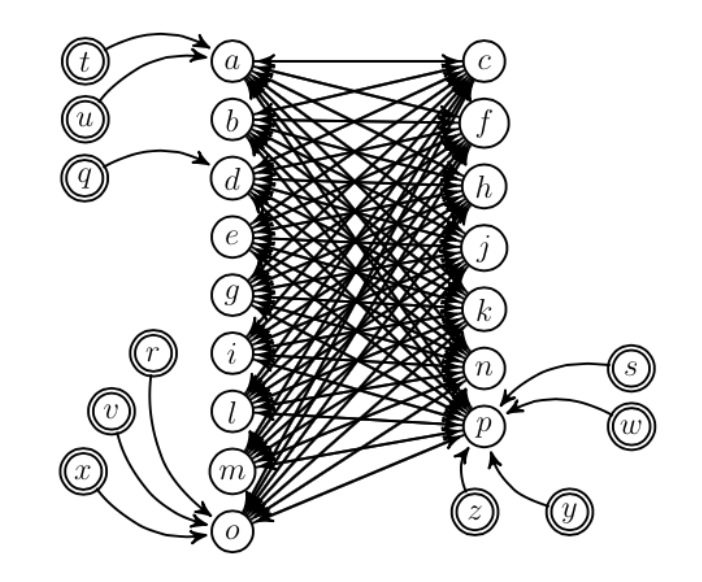
\includegraphics[width=0.5\textwidth]{argumentationframework}
\end{figure}

Dung modelled this interaction mathematically as a directed graph; with nodes representing the arguments and edges representing the attack relations between the arguments. This model of arguments and attack relations is known as an argumentation framework.

Within an argumentation framework an argument A can become inadmissible if it is attacked by another argument B. However, if B is attacked by C and becomes in admissible then A may be reinstated.

\begin{figure}[h]
\centering
\begin{tikzpicture}

\tikzset{vertex/.style = {shape=circle,draw,minimum size=1.5em}}
\tikzset{edge/.style = {->,> = latex'}}
% vertices

\node[vertex] (a) at  (0,0) {$a$};
\node[vertex] (b) at  (1.5,0) {$b$};
\node[vertex] (c) at  (3,0) {$c$};

%edges

\draw[edge] (c)  to[bend left] (b);
\draw[edge] (b)  to[bend right] (a);

\end{tikzpicture}
\caption{A is reinstated since C attacks B}
\end{figure}


\subsection{Semantics}

\subsection{Admissible Defense Sets}

\cite{vreeswijk2006algorithm}

\subsection{Knowledge Elicitation}

In order to develop expert systems a knowledge engineer must gather domain expertise. This knowledge is elicited in a number of ways. Typically the knowledge engineer is not an expert in the domain and will gather the knowledge from books, journals and other sources. It may be more efficient for the knowledge engineer to elicit a knowledge base directly from an expert by interviewing them. Although this approach is preferable it is not always possible as the expert is busy with other work and unavailable for the long periods of time required to build a knowledge base.



\subsection{Argumentation Theory Implementations}
\label{sec:dr_implementations}

\cite{modgil2014aspic+} presented a tutorial introduction to ASPIC+; a framework for structured argumentation that is meant to generate abstract argumentation frameworks similar to those described by Dung. Within their framework arguments could be attacked in three ways: their uncertain premises, their defeasible inferences or on the conclusions of their defeasible inferences. The authors claim that Dungs calculus is indispensable, it provides little guidance for the modelling of such a system. ASPIC+ is proposed as a framework to guide the implementation of such a system, but is not itself implemented.

Computers can be used to model arguments using visualisation techniques. An example of this is argument diagramming tools; effective aids in helping people reason about arguments. Araucaria is one such tool is described by Reed and Rowe (2001). Araucaria was designed to make argument diagramming for undergraduates easier and also to support research activities. Reed and Rowe also developed AML (Argument Markup Language) an XML based syntax for describing the structure of arguments. Unlike Dung’s argumentation framework, Araucaria represents arguments in a tree structure and the branches of this tree represent support relations as opposed to defeat relations.

Implementations of argumentation systems are more commonly based around decision support systems. A review of defeasible reasoning implementations by Bryant and Krause (2004) highlight the need for well designed empirical evaluations of implementations and formal complexity analysis to justify the practical applicability of a reasoning engine. The paper also highlights the proprietary nature of successful argumentation theory based applications preventing researchers from peer reviewing the software.

Karacapilidis and Papadias (2001) describe HERMES, a system for computer supported argumentation and decision making. HERMES also provides users with access to information from external databases to further justify their arguments. Arguments are represented using a labelling approach as opposed to a graph approach. Constraints are inserted into a discussion graph and when new constraints are introduced they are checked against existing ones.

The fact that decision support systems allow users to aggregate evidence and make decisions based on that evidence lends makes them an obvious fit for medical practitioners. Hunter and Williams (2010) developed a framework for generating inference rules to argue for and against the benefits of medical treatments based on evidence. Their work highlights the benefits of argumentation systems in abstracting away the complicated nature of medical evidence into a form more manageable for practitioners.

Longo and Hederman (2013) similarly investigated the role of argumentation theory in the implementation of decision support systems. Their work provides a comparison with machine learning. The authors developed an argumentation framework (similar to to those described by Dung) to model the breast cancer recurrence problem. The results of their experiment showed that argumentation based systems could perform as well and in some cases better than machine learning algorithms.


\section{Argument Maps Improve Critical Thinking}



%----------------------------------------------------------------------------------------
%	EVALUATION
%----------------------------------------------------------------------------------------
\section{Evaluation}
\label{sec:evaluation}
As the overall aim of the research project is to compare an implementation of defeasible reasoning with machine learning, a framework for comparing the two must be developed. This is no easy task as the techniques vary considerably in the output they will produce. For supervised machine learning the output of the experiment will be a number or a classification. These numbers and classes will already be present in the training and test data sets. For defeasible reasoning this is not the case. The implementation outputs a value that is a representation of a construct. In the experiments performed for this project, that construct is mental workload. There are many ways to measure mental workload but there is no one definitive value that can be used for comparison with this value. There is no value already present in the dataset that we can compare the output of the defeasible reasoning system with.

The following section gives an overview of the various methods used to evaluate the techniques in work by previous authors.

\subsection{Evaluation of Machine Learning Techniques}\cite{witten2005data}

There are a number of methods typically used for evaluation of machine learning techniques. Numeric predictions are evaluated similarly to many scientific experiments using statistical values such as correlation and mean absolute error. Machine learning techniques for solving classification problems are often more detailed as the costs of false positives and false negatives may be different depending on the problem. Take for example the prediction of cancer recurrence. A false positive (that it is predicted cancer will recur when it will not) will result in a patient being examined by a doctor; on the other hand a false negative would result in the missed opportunity of early diagnosis, potentially costing a life.

Machine learning techniques are typically evaluated first developing a model using a labeled `training set' of data. Once the model has been developed it can be run on a labeled `test set' of data. The performance of the technique can then be measured by comparing the values predicted by the model with the labels in the test set. The exception to this is with unsupervised machine learning as the data is unlabeled. As the purpose of unsupervised machine learning is to come up with a kind of `theory' about the data, good techniques ``make everything as simple as possible, but not simpler''. This idea is the foundation of the Minimum Discription Length Principle.

Typically the amount of data used for training and testing is limited and so techniques such as cross validation and percentage of split may be used to test and validate the model. In percentage of split the data set is divided into two groups, one for training and one for testing. Typically a higher percentage is used for training the data than testing it. In cross validation a data set is divided into groups. One group is used at a time for testing the model while the rest of the data in the set is used for training it. This technique is often referred to as N-fold cross validation where N is the number of groups the data is divided into. 

The following is a brief description of a number of measures used when evaluating the results of machine learning techniques.

\subsection{Numeric Prediction Problems}

\cite{witten2005data} explain that for practical situations the best numeric prediction method tends to perform well across all performance measures. Most performance measures tend to give an overall value for the difference between the predicted and actual value in a test set. Examples of such measure include mean-squared error, root mean-squared error and mean absolute error. As mean squared error squares the difference from the mean it tends to punish large errors more than the other measures.

Mean-squared error can be defined:

$$\frac{\sum \limits_{i=1}^n (p_{i} - a_{i})^2}{n}$$

Where $p$ are the predicted values and $a$ are the actual values.

Another performance measure used for numeric prediction problems is Pearson's Correlation Coefficient. This measures the linear correlation between the predicted value and the actual value. It differs from the other measure in that it ignores the differences in the scale of the two values.

$$\frac{S_{PA}}{\sqrt{S_{P}S_{A}}}$$

where:

$$S_{PA} = \frac{\sum _{i}(p_i - \bar{p})(a_i - \bar{a})}{n - 1}$$

$$S_{P} = \frac{\sum _{i}(p_i - \bar{p})^2}{n - 1}$$
$$S_{A} = \frac{\sum _{i}(a_i - \bar{a})^2}{n - 1}$$


\subsection{Classification Problems}

\subsection{Unsupervised ML - Minimum Description Length}

\cite{grunwald2005tutorial} gives an overview of how the Minimum Description Length Principal is used to solve the problem of model selection. Overfitting is a problem that occurs frequently with unsupervised ML techniques. Overfitting occurs when a learning technique puts too much emphasis on fitting the data exactly. As a result data points like outliers can skew the model and result in it classifying future instances of the data wrongly. A model that overfits the data will classify the dataset used to train it with very little error, however, when used on a test set will perform poorly. A simpler model may not classify the training data perfectly but will perform better on test data.

As observed earlier, a simpler theory is one that allows data to be encoded using fewer bits. This idea is born from information theory. For example, the SVG file type encodes a red circle as \lstinline{<circle cx="50" cy="50" r="40" stroke="black" stroke-width="3" fill="red" />}. This is far simpler than sending every single bit used to describe circle in raw data. From the perspective of programming MDL can be compared to Kolmogorov Complexity; the simplest theory is the one that produces the shortest computer program that will print the data.

MDL views learning as data compression; \cite{grunwald2005tutorial} defines this formally: ``for a given set of hypotheses H and data set D, we should try to find the hypothesis or combination of hypotheses in H that compresses D most.'' The best point hypothesis H to explain the data D is the one which minimizes the sum L(H) + L(D|H), where
\begin{itemize}
  \item L(H) is the length, in bits, of the description of the hypothesis; and
  \item L(D|H) is the length, in bits, of the description of the data when encoded
\end{itemize}
with the help of the hypothesis.

With this in mind it can the simple representation of constructs should be considered favourable to one that is complex.

\subsection{Evaluation of Defeasible Reasoning Implementations}

The HERMES system\cite{karacapilidis2001computer} is an implementation of Argumentation Theory that allows users to collaboratively develop arguments online and support those arguments with data. The authors evaluated their system focusing on usability. A wide variety of users such as students, researchers and medical doctors were surveyed. The participants attempted to solve two problems collaboratively using the tool and then answered questions. These questions were both about the users overall opinion of the system (ease of use, enjoyable, intention to use again) and about effectiveness of the system (task clarity, easy to read, sufficiently informative). The tool focuses on collaborative decision making and not on automated output so there is no evaluation of task performance.

Matt et al.\cite{matt2010combining} combined statistical methods with argumentation theory in order to compute trust.
%how did they do this and evaluate it?

%Discuss evaluation by longo and hederman
Generally when argumentation approaches are evaluated researchers compare the ability of the implementation to predict a value already present in the dataset. 

%----------------------------------------------------------------------------------------
%	CONCLUSIONS
%----------------------------------------------------------------------------------------

\section{Conclusions}
